%%%%%%%%%%%%%%%%%%%%%%%%%%%%%%%%%%%%%%%%%%%%%%%%%%%%%%%%%%%%%%%%%%%%%%%%%%%%%%%%%%%%%%%%%%%%%%%%%%%%%%%%%%%
		\subsection{Notation}
%%%%%%%%%%%%%%%%%%%%%%%%%%%%%%%%%%%%%%%%%%%%%%%%%%%%%%%%%%%%%%%%%%%%%%%%%%%%%%%%%%%%%%%%%%%%%%%%%%%%%%%%%%%


\begin{frame}
		\frametitle{Getting inside Parallel Tempering}
	
	\begin{center}
	\begin{tabular}{cc}
		$(\Omega, \mathfrak{F})$ & measurable space \\ 
		 
		$\Omega$ & subset of a Polish space \\ 
		 
		$\mathfrak{F}$ & Borel subsets countably generated\\ 
		 
		$\mathcal{I} = [0,1]$ & unit interval \\ 
		 
		$ \pi: \mathfrak{F} \mapsto \mathcal{I}$ & measure \\ 
	\end{tabular} 	


		\begin{figure}\includegraphics[scale=.3, keepaspectratio]{./picts/nutshell2.jpg}\end{figure}	
	\end{center}

\end{frame}


%%%%%%%%%%%%%%%%%%%%%%%%%%%%%%%%%%%%%%%%%%%%%%%%%%%%%%%%%%%%%%%%%%%%%

\begin{frame}
		\frametitle{Assumptions and further notation}
	
	\begin{itemize}
		\item[\textcolor{green}{As.}] $\pi$ has density w.r. to Lebesgue measure
		\item $\pi$ - the density
		\begin{itemize}
			\item know up to its proportionality factor
			\item unnormalised
		\end{itemize}
	\end{itemize}	

	 $$ \int_{\Omega} \pi(x) \mathrm{d}\, x \in (0, \infty) $$
\end{frame}


%%%%%%%%%%%%%%%%%%%%%%%%%%%%%%%%%%%%%%%%%%%%%%%%%%%%%%%%%%%%%%%%%%%%%%%%%%%%%%%%%%%%%%%%%%%%%%%%%%%%%%%%%%%
		\subsection{Ideology}
%%%%%%%%%%%%%%%%%%%%%%%%%%%%%%%%%%%%%%%%%%%%%%%%%%%%%%%%%%%%%%%%%%%%%%%%%%%%%%%%%%%%%%%%%%%%%%%%%%%%%%%%%%%

\begin{frame}
		\frametitle{Solution's ideology}
	
	\begin{itemize}
			
		\item[] Space for chains
			 $$(\Omega^L, \mathfrak{F}^{\otimes L}, \pi_\beta)$$
		\item[]
		\item[] where $\mathfrak{F}^{\otimes L} \equiv \underbrace{\mathfrak{F} \otimes \dots \otimes \mathfrak{F}}_{\text{$L$ times}}$
		\item[]
		\item[] $$ \pi_\beta \propto \pi^{\beta_1} \times \dots \times \pi^{\beta_L} $$
		\item[]
		\item[] $\beta = (\beta_1 , \dots , \beta_L)$ - inverse temperatures $\beta_i = T_i^{-1}$
		\item[] and $1 = T_1 < \dots < T_L < \infty$	
		\item[]
		\item[]\emph{no normalisation of $\pi_\beta$ coordinates }	
	\end{itemize}	


\end{frame}

%%%%%%%%%%%%%%%%%%%%%%%%%%%%%%%%%%%%%%%%%%%%%%%%%%%%%%%%%%%%%%%%%%%%%

\begin{frame}
		\frametitle{\dots enters Markov}
	
	\begin{itemize}
			
		\item[] Markov Chain $X \equiv \{ X^{[k]}\}_{k \geq 0}$
		\begin{itemize}
			\item $\Omega^L$ state-space for $ X $
		\end{itemize}
		
		\item[]   $$X^{[k]} = (X_1^{[k]}, \dots, X_L^{[k]})$$
	\end{itemize}	

	\begin{center}
\begin{figure}\includegraphics[scale=1, keepaspectratio]{./picts/influence.pdf}\end{figure}	
	\end{center}
\end{frame}


%%%%%%%%%%%%%%%%%%%%%%%%%%%%%%%%%%%%%%%%%%%%%%%%%%%%%%%%%%%%%%%%%%%%%

\begin{frame}
		\frametitle{ non-Swedish way to equidistribution }
	
	\begin{itemize}
			
		\item[\textcolor{green}{As.}] $ \pi > 0$ somewhere between modes 
		
		\begin{itemize}
			\item then $\pi^{\beta_k} > \pi$ for $k \geq 2$
		\end{itemize}
		
		\item[] So that if $\pi(y) < \pi(x)$ then  
 $$\alpha_{\beta_1}(x,y) = 1 \wedge \frac{\pi(y)}{\pi(x)} = \frac{\pi(y)}{\pi(x)} <  \Big(\frac{\pi(y)}{\pi(x)}\Big)^{\beta_k} = 1 \wedge (\frac{\pi(y)}{\pi(x)})^{\beta_k} = \alpha_{\beta_k}(x,y)$$

		\begin{itemize}
			\item proposal accepted more often in higher temperatures when  $$\frac{\pi(y)}{\pi(x)} < 1$$
			\item we enlarge regions from which proposals get accepted
		\end{itemize}

	\end{itemize}	

\end{frame}


%%%%%%%%%%%%%%%%%%%%%%%%%%%%%%%%%%%%%%%%%%%%%%%%%%%%%%%%%%%%%%%%%%%%%%%%%%%%%%%%%%%%%%%%%%%%%%%%%%%%%%%%

\begin{frame}[plain]

	\begin{center}
		\begin{figure}\includegraphics[scale=.15]{./picts/Liang_perspectives.png}\end{figure}	
	\end{center}	
		
\end{frame}


\begin{frame}[plain]

	\begin{center}
		\begin{figure}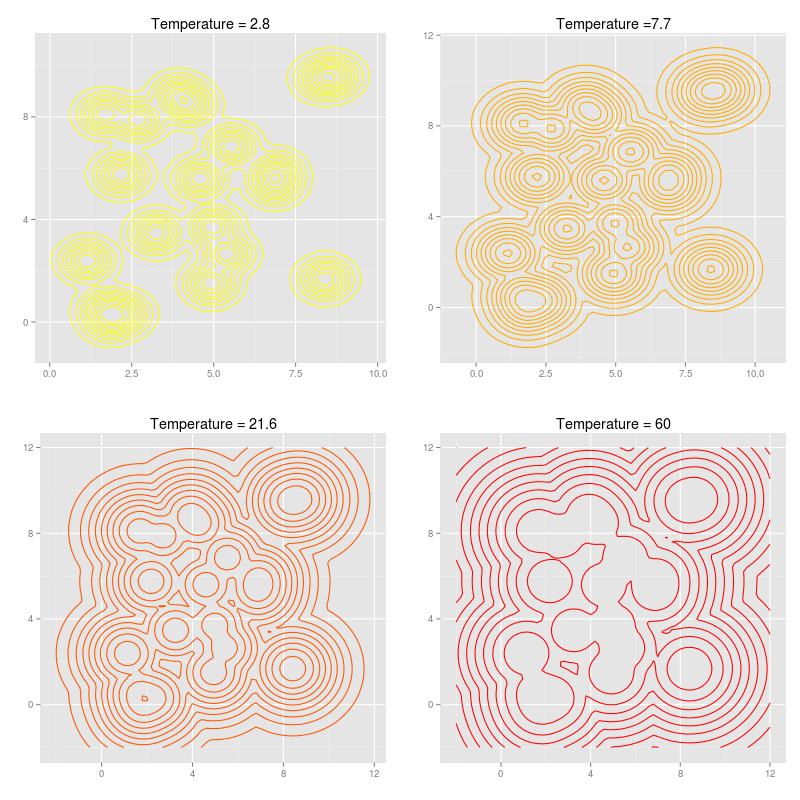
\includegraphics[scale=.31]{./picts/Liang_Contour_plots.png}\end{figure}	
	\end{center}	
		
\end{frame}

%%%%%%%%%%%%%%%%%%%%%%%%%%%%%%%%%%%%%%%%%%%%%%%%%%%%%%%%%%%%%%%%%%%%%

\begin{frame}
		\frametitle{ Potential Problems }

	\begin{center}
		\begin{figure}\includegraphics[scale=1, keepaspectratio]{./picts/probability_cloud1.pdf}\end{figure}	
	\end{center}
\end{frame}


%%%%%%%%%%%%%%%%%%%%%%%%%%%%%%%%%%%%%%%%%%%%%%%%%%%%%%%%%%%%%%%%%%%%%

\begin{frame}
		\frametitle{ Potential Problems }

	\begin{itemize}
		\item $\pi$ might be ok 
		\item because of computer's finite arithmetic it is not ok anymore
	\end{itemize}

\end{frame}


%%%%%%%%%%%%%%%%%%%%%%%%%%%%%%%%%%%%%%%%%%%%%%%%%%%%%%%%%%%%%%%%%%%%%

\begin{frame}
		\frametitle{ Theoretical Details }

	\begin{itemize}
		\item[] algorithm reached $n^\text{th}$ step - $X^{[n]}$
		\item[] we act with two kernels
 $$X^{[n]} \overset{\swap}{\rightarrow} \widetilde{X}^{[n +1]} \overset{\metro}{\rightarrow} X^{[n + 1]}.$$
		
		\item[]
		\item $\swap$ - swap kernel
		\item $\metro$ - random walk kernel
		\item[]
		\item Their reversibility is assured by the MHG algorithm reversibility. 
		\begin{itemize}
			\item[] so we get $\pi$-preservation 
			$$ \swap \metro \pi =  \swap \pi = \pi$$
		\end{itemize}
	\end{itemize}

\end{frame}
%%%%%%%%%%%%%%%%%%%%%%%%%%%%%%%%%%%%%%%%%%%%%%%%%%%%%%%%%%%%%%%%%%%%%%%%%%%%%%%%%%%%%%%%%%%%%%%%%%%%%%%%%%%
		\subsection{random walk kernel}
%%%%%%%%%%%%%%%%%%%%%%%%%%%%%%%%%%%%%%%%%%%%%%%%%%%%%%%%%%%%%%%%%%%%%%%%%%%%%%%%%%%%%%%%%%%%%%%%%%%%%%%%%%%

\begin{frame}
		\frametitle{ random walk $\metro$ }

	\begin{itemize}
		\item[] take $A_i \in \mathfrak{F}$ and $x \in \Omega^L$
		\item[] then
  $$\metro (x, A_1 \times \dots \times A_L) = \prod_{l=1}^L \metrobis{l}(x_l, A_l)$$
		
		\item[] where $\metrobis{l}(x_l, A_l)$ is equal to  
		\item[] 
$$\int_A \alpha_{\beta_l} (x_l, y_l) q_{\Sigma_l} (y_l - x_l) \mathrm{d }y_l + \delta_x (A) \int [1 - \alpha_{\beta_l} (x_l, y_l)] q_{\Sigma_l} (y_l - x_l) \mathrm{d }y_l$$

		\item[] where $\alpha_{\beta_l}$ is the acceptance level 
		\item[] and $q_{\Sigma_l}$ is proposal distribution 
	\end{itemize}

\end{frame}

%%%%%%%%%%%%%%%%%%%%%%%%%%%%%%%%%%%%%%%%%%%%%%%%%%%%%%%%%%%%%%%%%%%%%
\begin{frame}
		\frametitle{ Observations and assumptions }

	\begin{itemize}
		\item[\textcolor{green}{As.}] $q_{\Sigma_l}$ - density of $\mathcal{N}(0, \Sigma_l)$
		\item[]
		\item[] Symmetry $q(x_l,y_l) = q(y_l,x_l)$ implies 
		\item[]	$$ \alpha_{\beta_l} (x_l, y_l)  \equiv 1 \wedge \frac{\pi^{\beta_l}(y_l)}{\pi^{\beta_l}(x_l)} $$
		\item[] for the chain to preserve $\pi_\beta$.
		\item[] 
		\item[] Implementation: independent simulation of $\metrobis{l}$ for each $\widetilde{X}^{[n-1]}_l$
		
	\end{itemize}

\end{frame}

%%%%%%%%%%%%%%%%%%%%%%%%%%%%%%%%%%%%%%%%%%%%%%%%%%%%%%%%%%%%%%%%%%%%%%%%%%%%%%%%%%%%%%%%%%%%%%%%%%%%%%%%%%%
		\subsection{swap kernel}
%%%%%%%%%%%%%%%%%%%%%%%%%%%%%%%%%%%%%%%%%%%%%%%%%%%%%%%%%%%%%%%%%%%%%%%%%%%%%%%%%%%%%%%%%%%%%%%%%%%%%%%%%%%

\begin{frame}
		\frametitle{ Interlacing independent chains with $\swap$}

	\begin{itemize}
		\item[] Swaps
		\begin{itemize}
			\item Less-tempered chains placed in unusual places
			\item a pair of coordinates $(\widetilde{X}^{[n-1]}_l, \widetilde{X}^{[n-1]}_k)$ drawn at random
			\item[\textcolor{green}{As.}] only one pair per turn
			\item different strategies possible 
		\end{itemize}

		\item[] 
		\item[]	Introduce swap operation 
		$$S_{ij} x = (x_1, \dots, x_{i-1}, x_j, x_{i+1}, \dots, x_{j-1}, x_i, x_{j+1}, \dots, x_L)$$
	\end{itemize}

\end{frame}

%%%%%%%%%%%%%%%%%%%%%%%%%%%%%%%%%%%%%%%%%%%%%%%%%%%%%%%%%%%%%%%%%%%%%
\begin{frame}
		\frametitle{ Precise kernel form of $\swap$}

	\begin{itemize}
		\item[] For any $x \in \Omega^L$ and $A \in \mathfrak{F}^{\otimes L}$ 
	$$\swap(x, A) \equiv$$
		\item[]
$$\underset{ i < j}{\sum} p_{ij}(x) \alpha_\text{swap} (x, S_{ij}x) \mathbb{I}_A(S_{ij} x) + \Big( 1 - \underset{ i < j}{\sum} p_{ij}(x) \alpha_\text{swap} (x, S_{ij}x)\Big) \mathcal{I}(x,A)$$

		\item[] where 
$$\alpha_\text{swap}(x,S_{ij} x) = \Big[  \Big(\frac{\pi(x_j)}{\pi(x_i)} \Big)^{\beta_i - \beta_j}  \frac{ p_{ij}(S_{ij} x )}{ p_{ij}( x ) }\Big] \wedge 1$$
		\item[] is the acceptance level for swaps, 
		\item[] $p_{ij}( x )$ - probability function of a swap given $x$. 
		\item[] \emph{Nota bene:} given state $x$, $\swap$ has a finite support 
	$$\mathfrak{S}_x \equiv\{ S_{ij} x : i <j \}$$
	\end{itemize}

\end{frame}


